\chapter{La domestication d'une machinerie virale complexe par des guêpes parasitoïdes}
{\hypersetup{linkcolor=GREYDARK}\minitoc}
\label{chap:intro-parasitoids}

\section{Les Hyménoptères parasitoïdes}

Un parasite désigne un organisme appartenant à une espèce qui profite d’un autre organisme (l'hôte) à ses dépens, parfois sans le tuer (par exemple le parasite de la malaria du genre \textit{Plasmodium}, les poux ou bien le VIH). Un insecte parasitoïde désigne un cas particulier de parasite mélangé à de la prédation puisque les larves se nourrissent à l’intérieur ou sur le corps d’autres arthropodes. Les larves du parasitoïde consomment donc leur hôte. Les guêpes parasitoïdes ont un aspect bien différent des guêpes jaune et noire que l’on connaît bien. Il s’agit plutôt de guêpes de petite taille, pouvant être assez minuscules pour passer à travers le chas d’une aiguille. Les plus grosses ne dépassent que très rarement les quelques cm. La majorité des insectes parasitoïdes est retrouvée au sein de l’ordre des Hyménoptères (dont font partie les guêpes, les abeilles et les fourmis par exemple). Cet ordre est considéré comme le plus diversifié au sein des insectes \citep{forbes_1_2018}, et il est très important sur le plan économique : il contient de nombreuses espèces pollinisatrices ainsi que de nombreuses espèces parasitoïdes qui tuent naturellement d’autres insectes ravageurs de cultures \citep{foottit_biodiversity_2009}. 

Selon une analyse phylogénétique récente, la transition vers le mode de vie parasitoïde s'est produite une seule fois entre le Permien et le Trias il y a 247 millions d'années \citep{peters_evolutionary_2017}, suivi par des épisodes de reversions vers le mode de vie libre, que l'on retrouve aujourd'hui chez les insectes sociaux par exemple. Aussi, la majorité de la diversité des Hyménoptères parasitoïdes se retrouve dans le clade "parasitoida"\citep{peters_evolutionary_2017}(\figurename{\ref{figure:diversite-parasitoid}}- n.7).\\

\begin{figure}[!htpbt]
\captionsetup{font=footnotesize}
 \centering
  \includegraphics[width=\linewidth,height=\textheight,keepaspectratio]{PhD-master/figures/Diversite_parasitoide.pdf}
\caption[Intro:Phylogénie des Hyménoptères]{\textbf{Phylogénie des Hyménoptères modifiée de \cite{peters_evolutionary_2017}}.}
\label{figure:diversite-parasitoid}
\end{figure}

\textbf{Le cycle de vie des guêpes parasitoïdes}

Comme illustré dans la (\figurename{\ref{figure:cycle-de-vie}}), après accouplement, la femelle dépose ses œufs à l’intérieur d’un hôte (on appelle alors ces guêpes des endoparasitoïdes), ou à la surface de l’hôte (on les appelle alors guêpes ectoparasitoïdes). L'hôte est souvent attaqué durant les stades immatures (œufs, larves, pupe) bien que certains parasitoïdes attaquent les adultes. Les œufs puis les larves se développent alors dans ou sur l'insecte hôte jusqu'au dernier stade larvaire, puis chez certaines espèces, les larves sortent de l’hôte pour former une pupe (l’équivalent de la chrysalide chez les papillons), tandis que d'autres forment leur pupe à l'intérieur de l'hôte. Enfin, les adultes émergent de ces pupes, laissant derrière eux dans la grande majorité des cas leur hôte mort. Les espèces hôtes attaqués par ces guêpes sont extrêmement diversifiées. On peut dire que tous les arthropodes à tout stade de vie sont susceptibles d’être parasités par une ou plusieurs espèces de guêpes parasitoïdes \citep{capinera_carabid_2008}. Une guêpe parasitoïde en développement peut, elle-même, être attaquée par un autre parasitoïde, on parle alors d’hyper-parasitoïdisme. 

\begin{figure}[!htpbt]
\captionsetup{font=footnotesize}
 \centering
  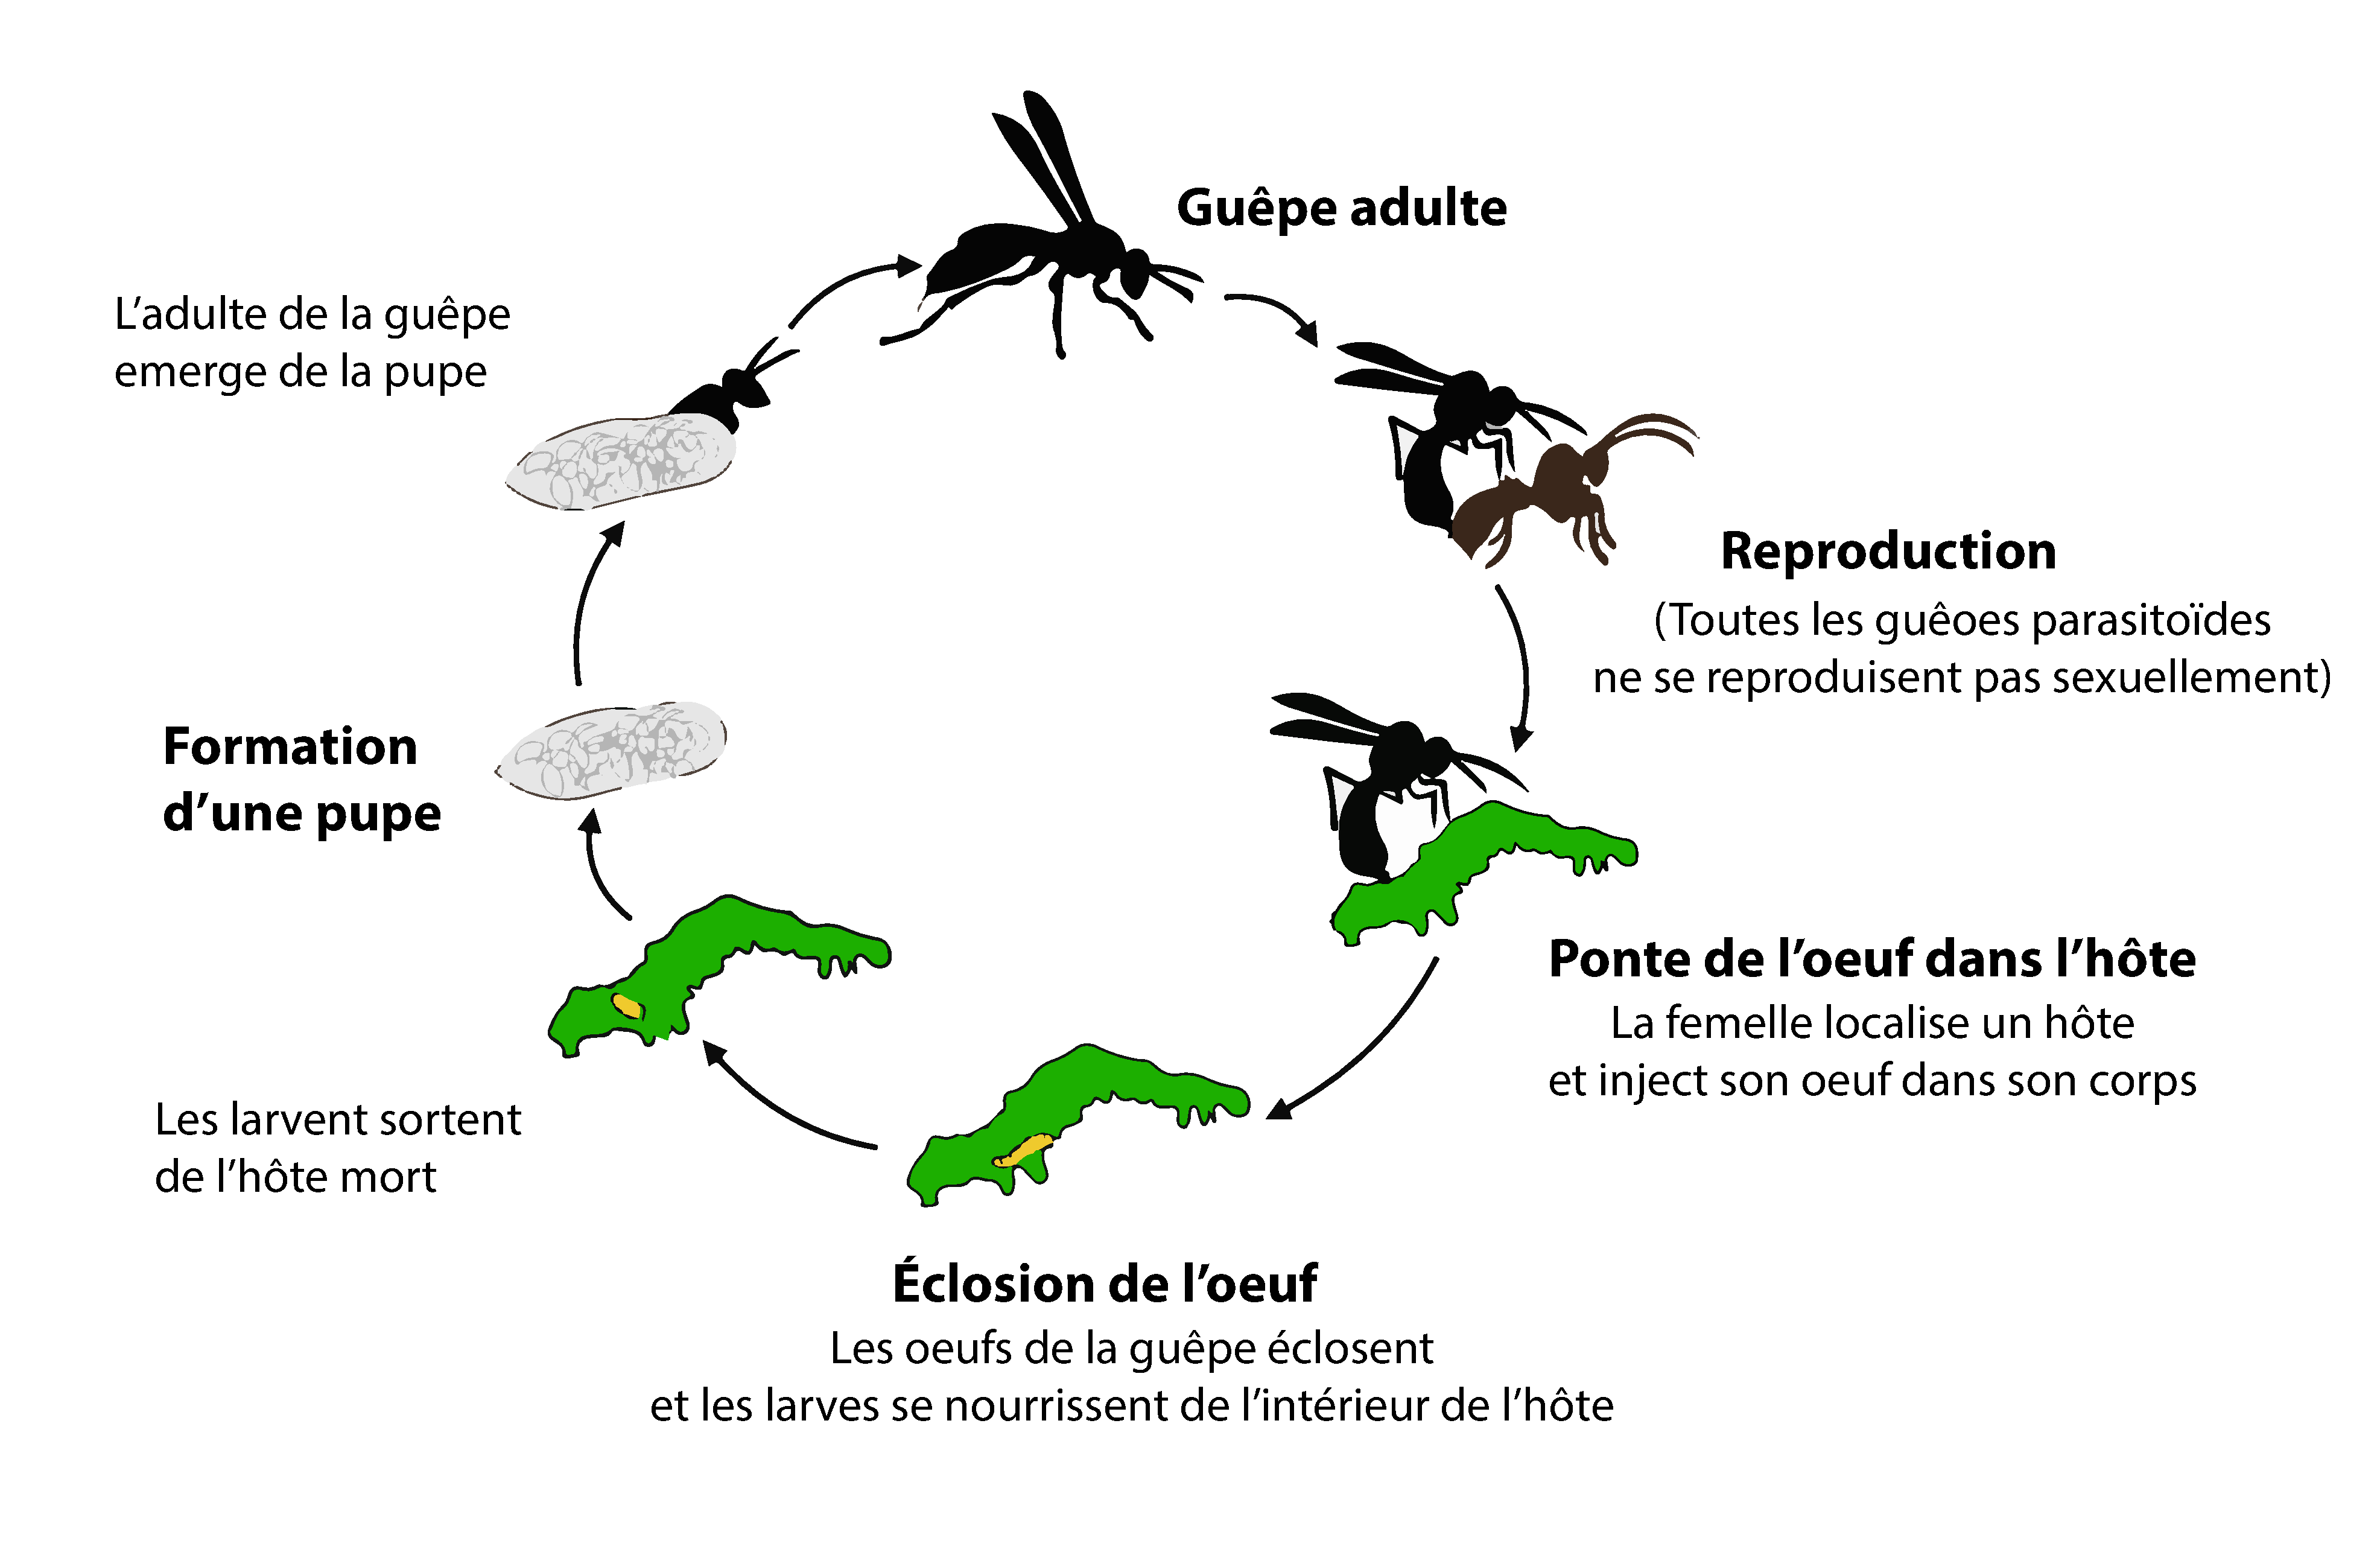
\includegraphics[width=\linewidth,height=\textheight,keepaspectratio]{PhD-master/figures/cycle-de-vie.pdf}
\caption[Intro:Cycle de vie général d'une guêpe endoparasitoïde]{\textbf{Cycle de vie général d'une guêpe endoparasitoïde} modifié de ce \href{https://www.sciencelearn.org.nz/resources/2770-parasitoid-wasp-life-cycle}{site}.}
\label{figure:cycle-de-vie}
\end{figure}

\section{Parasitoïdisme, une lutte incessante du parasitoïde contre son hôte}

Face aux parasitoïdes, les insectes  attaqués réagissent à travers une réponse immunitaire cellulaire. L'une des réponses les plus claires à l'infection par les guêpes est l'encapsulation de l'œuf de guêpe ou de l'embryon précoce. Cette réaction immunitaire innée a été documentée chez de nombreux arthropodes \citep{brehlin_immune_1988}. Par exemple, chez \textit{D.melanogaster}, l'injection d'un œuf de parasitoïde déclenche la production de davantage de plasmatocytes, de lamellocytes et une activation de la cascade de la phénoloxydase (PO) \citep{kim-jo_drosophila_2019}. Les plasmatocytes vont alors former une première couche de cellules autour de l'œuf de parasitoïde à laquelle les lamellocytes adhérent, formant ainsi des jonctions serrées pour former une capsule multicouche mélanisée. La cascade de PO produit ensuite des radicaux cytotoxiques, ce qui entraine la mort de l'œuf du parasitoïde \citep{kim-jo_drosophila_2019} (\figurename{\ref{figure:Encapsulation_process}}). 

\begin{figure}[!htpbt]
\captionsetup{font=footnotesize}
 \centering
  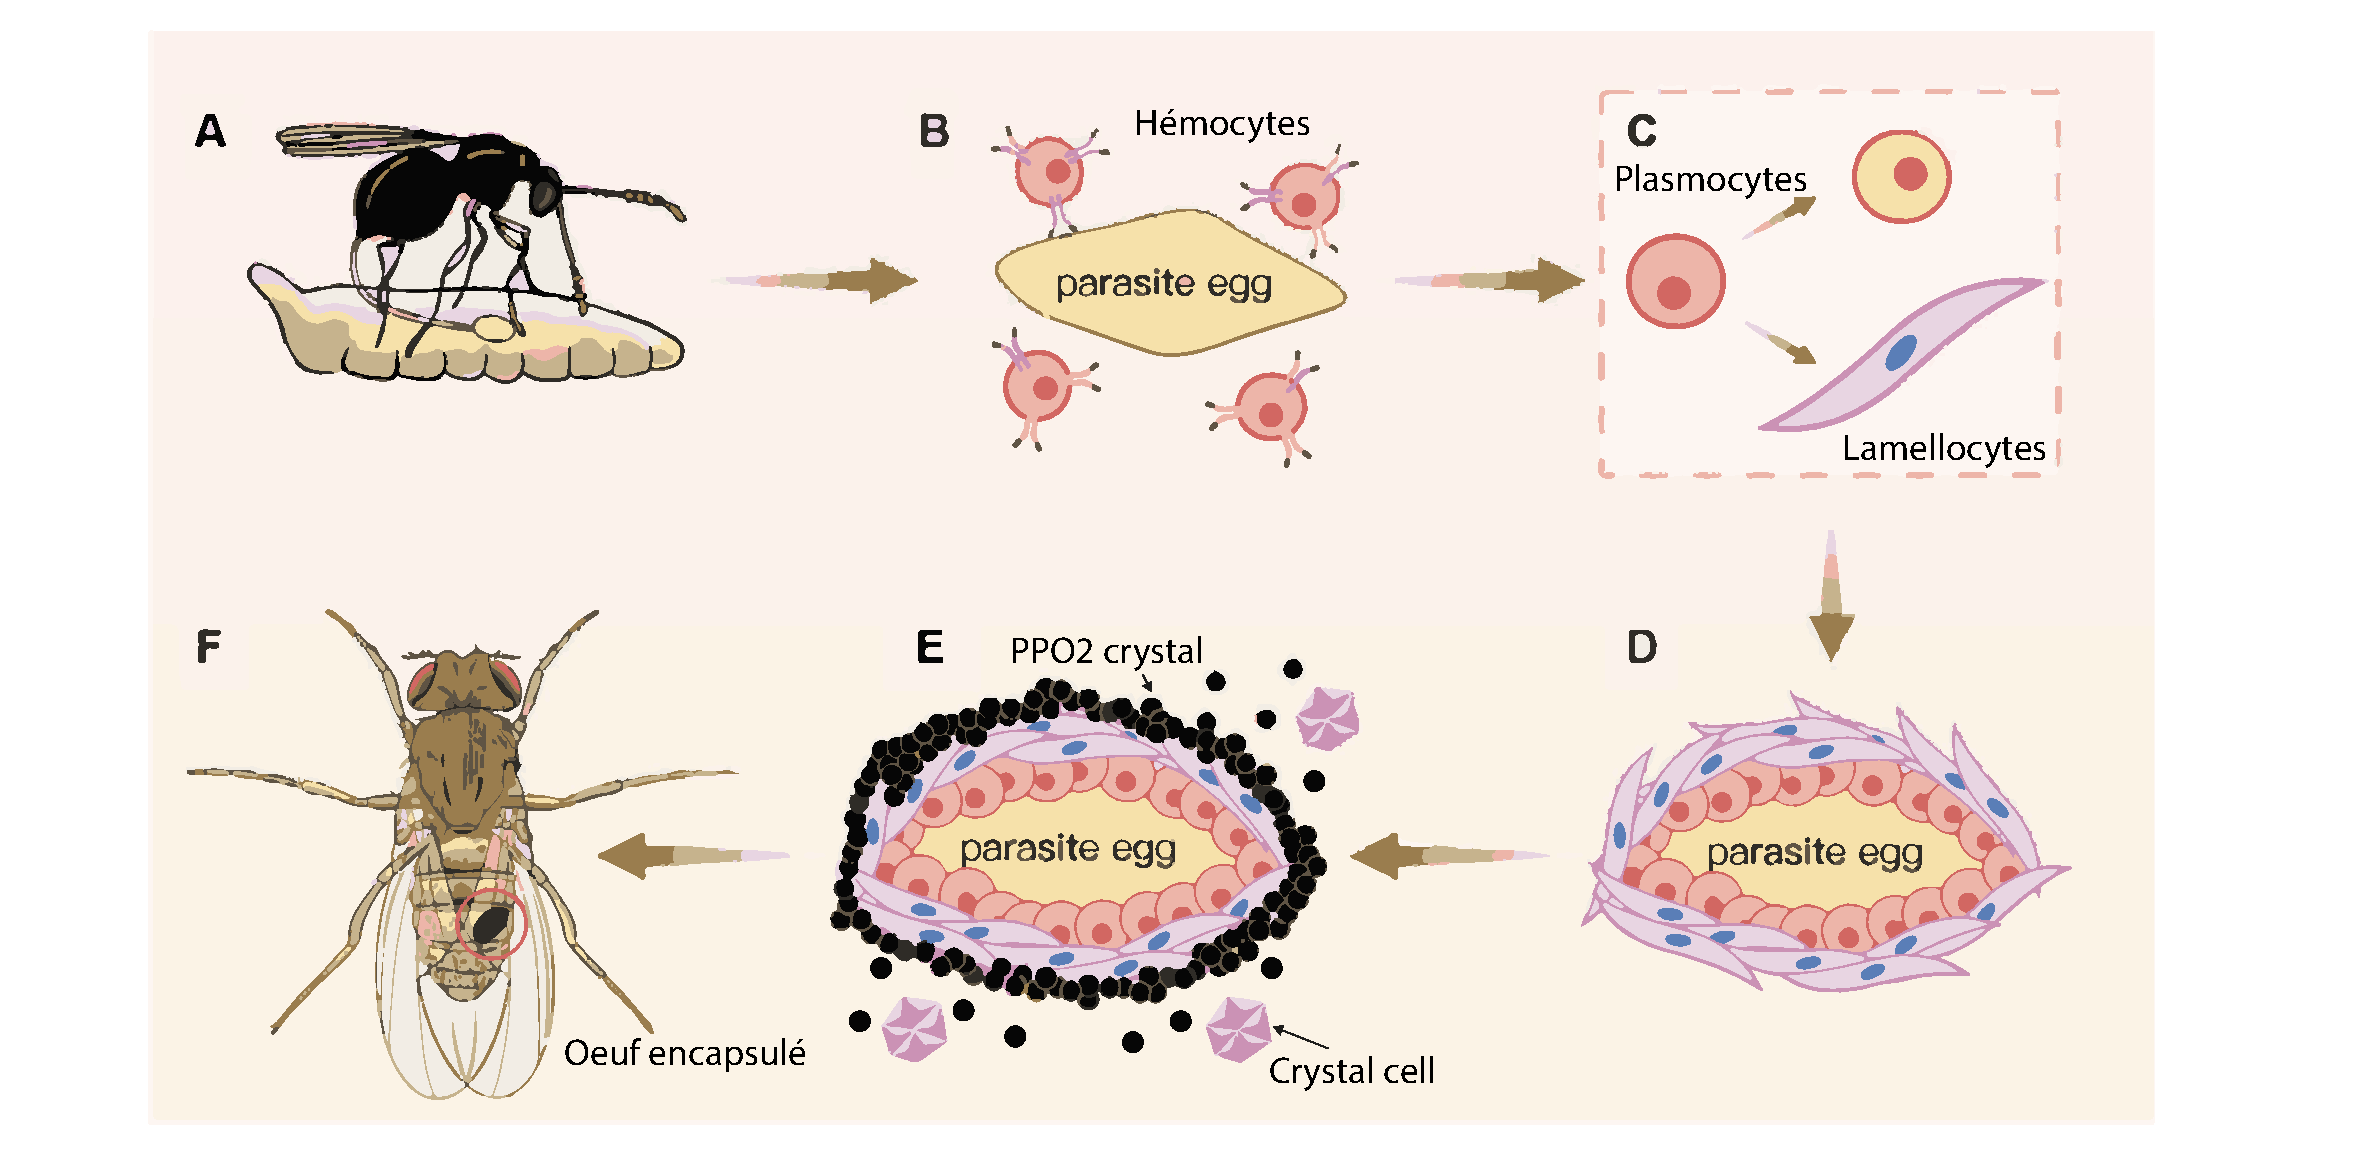
\includegraphics[width=\linewidth,height=\textheight,keepaspectratio]{PhD-master/figures/Encapsulation_process.pdf}
\caption[Intro:Schéma d'encapsulation général chez la drosophile]{\textbf{Les réponses de défense immunitaire de la drosophile hôte à l'encapsulation des œufs de guêpe tiré de \cite{yang_cellular_2021}}. \textbf{A} - La guêpe pond ses œufs dans l'hémocoele de l'hôte. \textbf{B} - Reconnaissance du non-soi médiée par les hémocytes sur les œufs de guêpe.\textbf{C} - Le recrutement des hémocytes implique la prolifération des plasmatocytes et la différenciation des lamellocytes. \textbf{D} - Les plasmatocytes et les lamellocytes migrent vers les œufs et les isolent. La formation de la mélanisation entourant les œufs de guêpe. \textbf{F} -  La guêpe périt, tandis que la drosophile survit.}
\label{figure:Encapsulation_process}
\end{figure}


Face à ce parasitoïdisme, il existe une asymétrie entre les deux entités puisque le parasitoïde est exposé à chaque génération au système immunitaire de son hôte. À l'inverse, la probabilité pour l'hôte d'être parasitoïdé varie fortement dans le temps ou l'espace \citep{fleury_chapter_2009}. Ainsi, du côté des parasitoïdes, de fortes pressions de sélection s'exercent sur leur capacité à contourner l'immunité et à modifier la physiologie de leur hôte (deux caractéristiques clés impliquées dans leur succès reproducteur). Diverses stratégies de contournement du système immunitaire ont donc été sélectionnées au cours de l'évolution. 

La forme de défense active la plus courante est l’injection de toxines (venin) par la femelle parasitoïde dans l'hémolymphe de l'hôte pendant la ponte \citep{asgari_venom_2011, moreau_venom_2015}. Ces toxines ont alors pour fonction d'inhiber le système immunitaire de l’hôte ou d'interrompre son développement \citep{moreau_venom_2015}. 

En termes d'interactions, alors que les guêpes ectoparasitoïdes utilisent leur venin pour conserver la nourriture pour leurs progénitures via la paralysie, les guêpes endoparasitoïdes utilisent leur venin pour transformer les hôtes pour que leurs progénitures puissent vivre et se nourrir jusqu'à l'éclosion \citep{moreau_chapter_2009,schendel_diversity_2019}. De plus, plusieurs études montrent que les espèces ectoparasitoïdes interagissent moins avec le système immunitaire de leurs hôtes comparé à des espèces au style de vie endoparasitoïde qui sont elles complétement plongée dans le corps de leurs hôtes, là où se trouvent notamment toutes les cellules de l'immunité \citep{li_parasitism_2018}. Chez les endoparasitoïdes, sauf dans quelques cas où une paralysie transitoire a été observée, le venin n'a généralement pas d'effet paralysant sur l'hôte, mais a  plutôt un effet de répression du système immunitaire. Après l'endoparasitoïdisme, l'hôte se rétablit généralement en quelques minutes et jusqu'à une heure. Les endoparasitoïdes évitent d'induire une paralysie à long terme chez l'hôte et adoptent un mode de vie dit koïnobionte. Dans ce cas, l'hôte est maintenu en vie et poursuit son développement, le parasitoïde étant toujours à l'intérieur \citep{moreau_venom_2015}.\\

Dans de nombreux systèmes parasitoïde-hôte, l'injection de substances particulières au sein de ces venins maternels permet également d'assurer le succès du parasitoïde. L'origine de ces substances a longtemps été débattue dans la communauté scientifique et nous savons aujourd'hui qu'une partie provient de la domestication de virus chez certaines espèces de guêpes endoparasitoïdes. Afin d'illustrer ce cas particulier, je vous propose une courte rétrospective historique pour résumer cette découverte (inspirée de l'ouvrage \textit{Parasitoid Viruses : Symbionts and Pathogenes} \citep{strand_polydnavirus_2012}).\\

Les racines de la découverte que je m'apprête à exposer proviennent du chercheur britannique George Salt qui, en 1965, montre que les fluides produits dans le calice (organe situé à la base des ovaires chez certains parasitoïdes comme ici chez le braconidae \textit{Venturia canescens}) protègent les œufs de l’encapsulation. Étrangement, en 1967, Susan Rotheram observe chez la même espèce, que de nombreuses « particules » produites dans les cellules du calice s'accrochent aux œufs \citep{rotheram_immune_1967,noauthor_surface_1973}. Pour certains.es observateurs·rices de l’époque, il s'agissait de virus compte tenu de leurs structures et de leurs tailles. Plus tard, chez une autre espèce de Braconidae (\textit{Cardiochiles nigriceps}), un traitement à la DNAse permet de mettre en évidence la présence d'ADN à l'intérieur des particules observées \citep{vinson_particles_1975}. Par la suite, des analyses complémentaires chez plusieurs genres de parasitoïdes issues de la superfamille des Ichneumonoidea (\textit{Toxoneuron}, \textit{Microplitis}, \textit{Chelonus} et \textit{Campoletis}) montrent des différences morphologiques notables entre les particules observées selon les espèces. La littérature jusqu'au début des années 1990 a donc majoritairement conclu que les particules observées étaient des virus, car ils : 1) se répliquent dans les cellules du calice des guêpes, 2) ressemblent morphologiquement à des virus, 3) contiennent des acides nucléiques, 4) sont infectieux, et 5) contiennent des gènes qui sont transcrits après l'infection des hôtes \citep{fleming_polydnaviruses_1992,stoltz_viruses_1979}. C’est à ce moment-là que le nom de « virus-like », puis polydnavirus (PDVs) (car les particules sont composées de plusieurs molécules d'ADN) a été proposé pour décrire ces particules virales ayant l'apparence de virus. Par la suite, en 1984, l'établissement d’une nouvelle famille virale est proposé et validé par la communauté scientifique (les \textit{Polydnaviridae}) \citep{stoltz_polydnaviridae_1984}. C’est en 2004 que le premier génome de polydnavirus est séquencé chez le Braconidae \textit{Cotesia congregata}. Cette découverte va chambouler la vision des chercheurs.euses de l’époque. Étonnamment, à l’intérieur de ces particules, aucun ADN apparenté à des virus connu n'est retrouvé. À l'inverse, les cercles d'ADN codent très majoritairement des facteurs de virulence d'origine eucaryote \citep{espagne_genome_2004,desjardins_comparative_2008}. Le séquençage des particules révèle donc que les gènes essentiels à leur production ne sont pas contenus dans les particules. C’est ainsi qu’en 2009, \cite{bezier_polydnaviruses_2009} identifient et confirment, grâce à l'étude du transcriptomique et du protéome de \textit{Cotesia congregata} pendant la phase de production des particules, la présence d'un ensemble de gènes d'origine virale impliqués dans la production de ces particules. Ce virus endogène est par la suite baptisé bracovirus du nom de la famille d’Hyménoptère Braconidae chez qui ces séquences ont été décrites pour la première fois. 
Il devient alors assez clair que les PDVs sont incapables de se répliquer dans l'hôte comme le font tous les virus, mais font plutôt partie intégrante du génome des guêpes.\\

\section{Biologie des structures virales délivrant des facteurs de virulence}

Depuis 2009, de nombreuses études ont précisé notre compréhension de l'histoire de l'acquisition et de l'utilisation de ces particules virales chez les guêpes apparentées à \textit{Cotesia congregata}. Nous savons aujourd'hui que ces particules virales sont codées par des gènes provenant d'un virus ancien qui a été endogénisé chez l'ancêtre commun de plusieurs milliers d'espèces appartenant au complexe des microgastroïdes \citep{strand_polydnaviruses_2015}. 

Ces « virus » ou plutôt gènes viraux domestiqués sont transmis verticalement via les chromosomes de la guêpe \citep{bezier_polydnaviruses_2009}. Ces gènes ne suivent en revanche pas les différentes étapes d'un cycle de vie viral, qui consiste à infecter des cellules cibles et à produire une descendance en créant de nouvelles particules. En effet, ce virus n'est plus libre à proprement parler, car les gènes viraux impliqués dans la synthèse des "virus" sont présents en permanence dans le génome de la guêpe. De plus, l'ADN codant pour les protéines induisant la réplication, l'empaquetage et l'enveloppement des virions n'est pas présent dans les particules infectieuses : ces virus ne sont donc plus infectieux \citep{strand_polydnaviruses_2015}. En ce sens, ces particules ne sont pas des virus typiques ; il s'agit plutôt d'entités hybrides "mi-virus mi-guêpe". 

Les particules virales ainsi produites servent de véhicules à la guêpe pour délivrer des composants spécifiques (que nous appellerons "facteur de virulence") directement aux cellules du système immunitaire de l'hôte. Ces facteurs de virulence sous forme de cercles d'ADNs sont alors adressés aux cellules immunitaires, puis s'intègrent dans les chromosomes de la cellule pour être exprimés par la machinerie cellulaire de l'hôte. Ces facteurs sont cruciaux pour le succès parasitaire, car ils comprennent différents éléments qui modifient la physiologie de l'hôte, rendant ce dernier plus adapté au développement des progénitures de guêpes \citep{gauthier_recurrent_2018}. 

Les facteurs de virulences se trouvent sous forme de gènes dans des cercles d'ADN double brin produits par les guêpes. Ces gènes sont pour la plupart d'origine de la guêpe (e.g. lectines de type C, protéine tyrosine phosphatase (ptp), ankyrines (ank), Egf) \citep{desjardins_comparative_2008, gasmi_recurrent_2015,huguet_evolution_2012}, tandis que d'autres plus rares dérivent d'éléments transposables (TE) \citep{zhang_chromosome-level_2019, gauthier_chromosomal_2021}. La quantité et la nature des gènes présents dans les cercles varient considérablement entre les espèces de guêpes, ce qui s'explique probablement par des phénomènes d'adaptation à différents hôtes \citep{bezier_functional_2013,serbielle_evolutionary_2012, strand_polydnaviruses_2012,cerqueira_de_araujo_chelonus_2022,mao_complete_2022}.
Par exemple, le contenu génique des bracovirus des guêpes parasitoïdes des familles Microgastrinae, qui pondent leurs œufs au stade larvaire, est différent de celui du parasitoïde \textit{Chelonus inanitus} (Cheloninae) qui parasite son hôte au stade œuf \citep{weber_transcriptional_2007, mao_complete_2022, cerqueira_de_araujo_chelonus_2022}. 

Ces cercles qui renferment ces facteurs de virulence proviennent des segments proviraux le long du génome des guêpes. Les segments proviraux appartiennent à des unités qui sont amplifiées pendant la formation des particules dans les cellules du calice \citep{louis_bracovirus_2013, burke_microplitis_2015}. Parmi ces unités amplifiables (unités de réplication), certains segments sont excisés et circularisés par recombinaison spécifique, ce qui nécessite des jonctions de répétition directe (DRJ) à leurs extrémités \citep{beck_encapsidated_2011,desjardins_structure_2007}(\figurename{\ref{figure:polydnavirus_integration_mechanism}}).

Une fois formés, les cercles d'ADN sont empaquetés dans des particules virales qui s'accumulent dans le calice, puis sont injectées dans l'hôte avec les œufs pendant l'oviposition \citep{strand_polydnaviruses_2014}. Ces particules s'attachent ensuite aux cellules de l'immunité pour y libérer les cercles d'ADN.  Dans le cas de certains polydnavirus étudiés, la majorité des cellules cibles sont des cellules immunitaires, comme les hémocytes \citep{beck_novel_2007}, mais ces particules peuvent également pénétrer dans presque tous les tissus, y compris les cellules de l'intestin et les cellules nerveuses \citep{beck_novel_2007, muller_genome-wide_2021}. Quoi qu'il en soit, parmi ces cercles, la majorité vont s'intégrer dans les chromosomes des cellules immunitaires \citep{chevignon_cotesia_2018, muller_genome-wide_2021} où les facteurs de virulence codés s'y trouvent exprimés \citep{pruijssers_ptp-h2_2007} permettant \textit{in fine} d’éviter la réponse immunitaire de l’insecte hôte \citep{drezen_endogenous_2017}.

Les mécanismes d'intégration de ces cercles viraux à l'intérieur du génome de l'hôte commencent à être bien décrits. Elle se produit grâce à un motif porté par certains cercles appelé motif d'intégration de l'hôte (HIM)\citep{beck_encapsidated_2011,chevignon_cotesia_2018,muller_genome-wide_2021}. Les intégrations de ces cercles impliquent deux jonctions, appelées jonction 1 (J1) et jonction 2 (J2), situées dans le HIM. Ces motifs sont par ailleurs conservés entre les espèces \textit{C.vestalis} et \textit{C.vestalis}\citep{mao_complete_2022}. J1 et J2 correspondent aux séquences qui forment les extrémités des séquences virales lorsqu'elles sont intégrées dans l'ADN de l'hôte (\figurename{\ref{figure:polydnavirus_integration_mechanism}}).

\begin{figure}[H]
\captionsetup{font=footnotesize}
 \centering
  \includegraphics[width=\linewidth,height=\textheight,keepaspectratio]{PhD-master/figures/polydnavirus_integration_mechanism.pdf}
\caption[Intro:Mécanisme d'intégration des cercles d'ADN]{\textbf{Mécanisme d'intégration des cercles d'ADN}. Les cercles d'ADN proviennent de séquences provirales contenues dans le génome de la guêpe. Ces segments proviraux contiennent des facteurs de virulence (loci rouges). Après amplification des segments proviraux, les molécules d'ADN produites sont circularisées par un mécanisme de recombinaison spécifique au site impliquant des répétitions directes légèrement différentes correspondant aux extrémités des segments proviraux (jonctions de répétition directe 5' (DRJ) et jonctions de répétition directe 3' (DRJ) : jaune et orange). La séquence circulaire comprend une DRJ circulaire (ou motif de jonction circulaire), une forme recombinée distincte des DRJ 5' et 3' (locus jaune/orange). De plus, les cercles d'ADN peuvent s'intégrer dans l'ADN génomique de l'hôte par un mécanisme impliquant très probablement une intégrase puis médié par des motifs d'intégration de l'hôte (HIM), indiqués par des lignes bleues. Une fois intégrés dans le génome, les facteurs de virulence vont être transcrits par la cellule hôte, et vont altérer la physiologie de la cellule, ce qui va l'empêcher de remplir sa fonction immunitaire.}
\label{figure:polydnavirus_integration_mechanism}
\end{figure}

De manière remarquable, d'autres espèces de guêpes parasitoïdes ont également domestiqué des virus de manière complètement indépendante. Dans tous les cas, ces virus domestiqués remplissent la même fonction biologique, c'est-à-dire qu'ils permettent de désactiver efficacement le système immunitaire de l'hôte.  Ainsi, selon l'espèce de guêpe, ces structures produites peuvent renfermer des facteurs de virulence sous forme de cercles d'ADN codant pour les gènes de virulence (chez les espèces connues pour produire des polydnavirus comme décrit plus haut, PDV)(\figurename{\ref{figure:PDV_VLP}}), ou sous forme de protéines (chez les espèces connues pour produire des protéines de type virales, VLP)(\figurename{\ref{figure:PDV_VLP}}). 

La propriété principale ayant été recrutée à plusieurs reprises, que ce soit chez les PDVs ou les VLPs est donc la capacité de fusionner les membranes (à l'image des \textit{syncitins} ou bien des gènes \textit{arc}) pour pénétrer à l'intérieur des cellules immunitaires de l'hôte. 

Dans les deux types de structures, toutes les fonctions majeures de l'ancêtre des virus domestiqués (excepté une réplication de l'ADN) ont été conservées : la transcription virale, l'empaquetage et l'infectivité \citep{drezen_endogenous_2017}. Les gènes impliqués dans la transcription virale au cours d'un processus infectieux, tels que les sous-unités de l'ARN polymérase virale (\textit{lef-4}, \textit{lef-8}, \textit{lef-9} et \textit{p47}), sont exprimés au début du développement nymphal de la guêpe et sont supposés réguler l'expression d'autres gènes viraux, tels que ceux codant pour les composants des nucléocapsides et des protéines d'enveloppe (\figurename{\ref{figure:PDV_VLP}}). 

\begin{figure}[H]
\captionsetup{font=footnotesize}
 \centering
  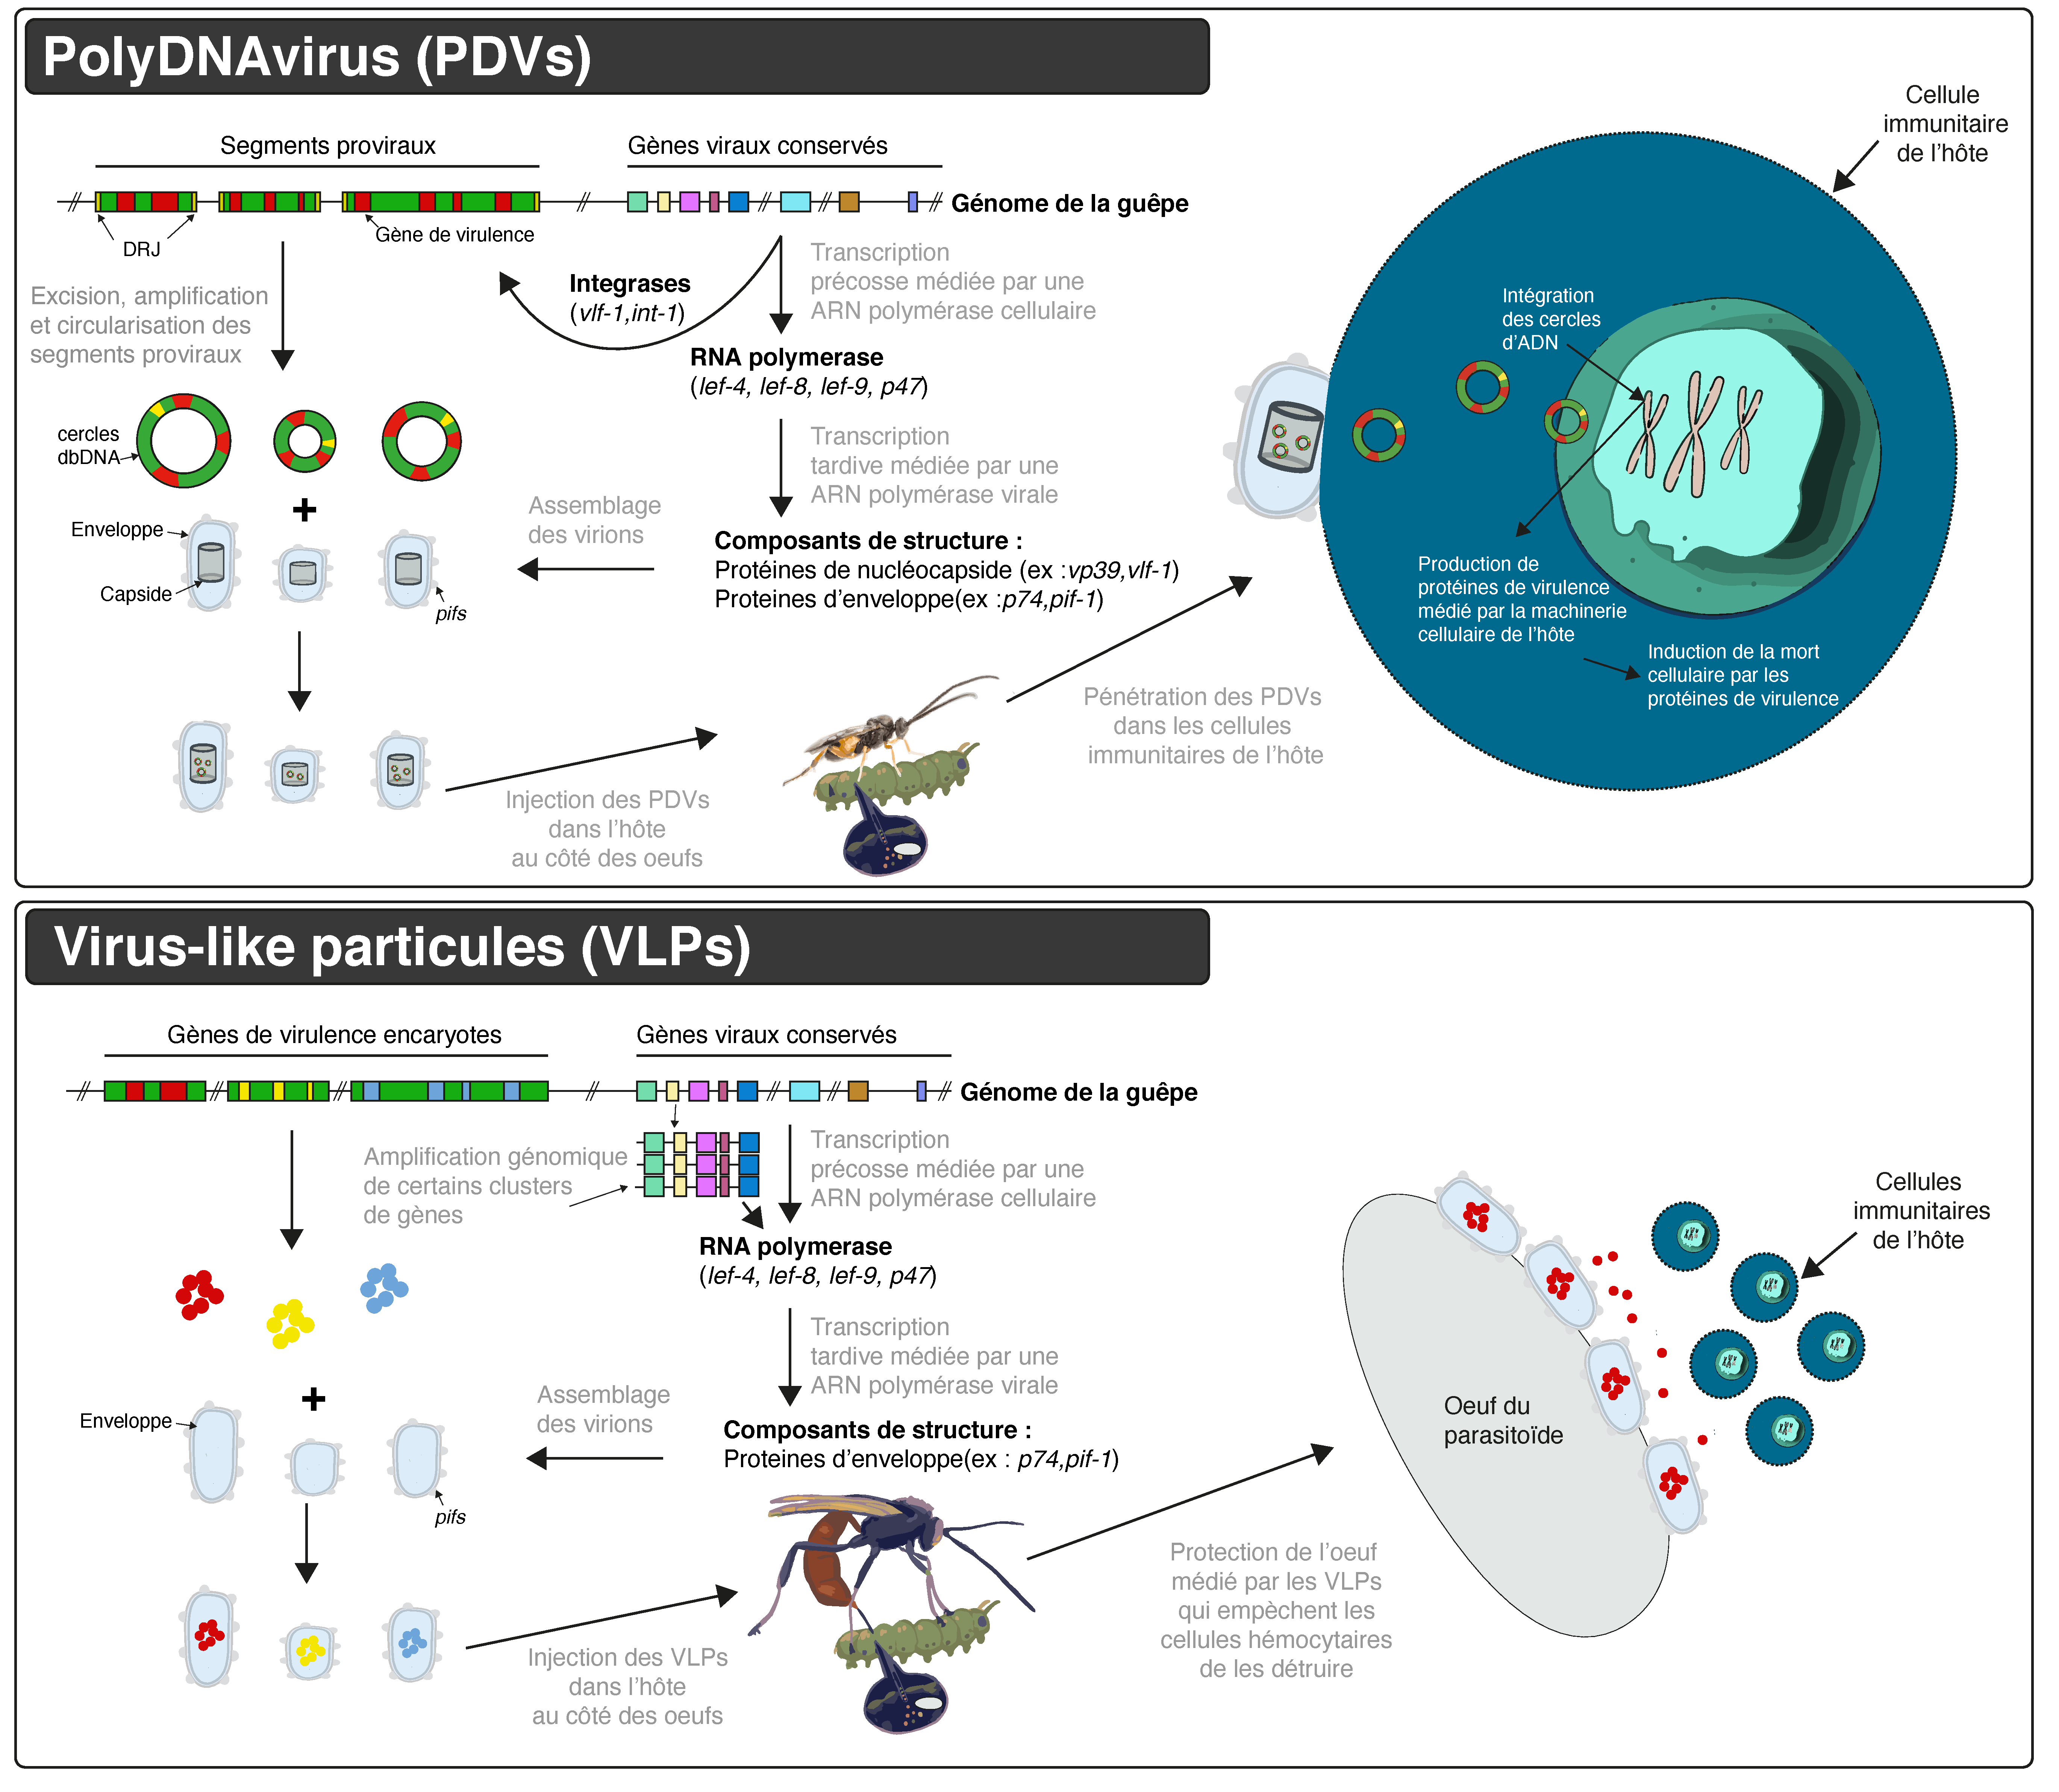
\includegraphics[width=\linewidth,height=\textheight,keepaspectratio]{PhD-master/figures/PDV_VLP.pdf}
\caption[Intro:Différentes structures à allures virales produites par les guêpes parasitoïdes]{\textbf{Différentes structures à allures virales produites par les guêpes parasitoïdes} }
\label{figure:PDV_VLP}
\end{figure}


\section{Les différents cas de domestications virales  chez les guêpes parasitoïdes}

Finalement, jusqu'à présent, six cas indépendants d'événements de domestication virale ont été rapportés, tous impliquant des donneurs de virus à ADN double brins de l'ordre des \textit{Lefavirales}. La plupart de ces événements de domestication se trouvent dans la super-famille des Ichneumonoidea, où 5 cas indépendants d'endogénisation virale sont décrits (\figurename{\ref{figure:Virus_arthropods_phylogeny}}-B). Le mieux documenté concerne l'intégration d'un génome nudiviral (grand virus à ADN double brin) il y a environ 100 millions d'années au sein du complexe des Microgastroïdes (Braconidea) qui contient des milliers d'espèces (on appelle les particules virales produites des bracovirus) (1) \citep{bezier_polydnaviruses_2009,whitfield_systematics_2018} (\figurename{\ref{figure:Virus_arthropods_phylogeny}}-B). Un autre exemple de polydnavirus implique 2 événements indépendants au sein des Ichneumonidea des sous-familles Banchinae (2) et Campopleginae (3) (on appelle les particules virales produites des ichnovirus) \citep{volkoff_analysis_2010,beliveau_genomic_2015}. Dans ce cas, les gènes qui permettent la production des particules virales contenant des cercles d'ADN sont regroupés dans des régions du génome de la guêpe (appelées IVSPERs) qui sont amplifiées lors de la réplication des particules virales, mais qui ne sont pas emballées dans les particules. Ces gènes ne présentent néanmoins pour l'heure aucune homologie de séquence dans les bases de données virales \citep{volkoff_analysis_2010}. Enfin, plus récemment, des cas de domestication de virus impliquant la production de VLPs ont été décrits chez l'espèce \textit{Venturia canescens} (bien qu'il s'agisse de l'espèce ou tout a commencé avec Rotheram et Salt) (4) \citep{pichon_recurrent_2015} et l'espèce \textit{Fopius arisanus} au sein de la sous-famille Opiinae (5) \citep{burke_rapid_2018}. \\

Bien que la super-famille des Ichneumonoidea soit la plus diverse des Hyménoptères \citep{klopfstein_darwin_2019,shimizu_integrative_2020}, elle ne représente qu'une petite partie de la diversité des Hyménoptères parasitoïdes \citep{forbes_1_2018} (\figurename{\ref{figure:diversite-parasitoid}}-B). D'autres espèces plus éloignées sont également concernées par ces phénomènes. En effet, nous avons récemment observé au sein du laboratoire que les VLPs produites par des guêpes appartenant à une super-famille très éloignée (6) (Cynipoidea) ont également une origine virale qui provient d'un virus proche de Leptopilina boulardi filamentous virus (LbFV), lui-même proche de la famille des \textit{Hytrosaviridae} (Di Giovanni et al., 2020) (\figurename{\ref{figure:Virus_arthropods_phylogeny}}-A). D'autres espèces de guêpes parasitoïdes dont \textit{Cotesia vestalis} (Braconidae) et \textit{Dolichomitus sp} (Ichneumonidae) présentent également des homologies de séquences avec des protéines de LbFV, bien qu'aucune preuve de leur domestication n'ait été rapportée jusqu'à présent \citep{burke_presence_2021}. Par ailleurs, d'autres cas d'endogénisations virales ont été décrits chez d'autres espèces d'Hyménoptères, comme au sein de la super-famille Chalcidoidea chez l'espèce \textit{Eurytoma brunniventris} \citep{zhang_chalcid_2020}, et même chez plusieurs espèces d'Hémiptères (\figurename{\ref{figure:Virus_arthropods_phylogeny}}-B). Cependant, aucune preuve de domestication n'a été trouvée chez ces dernières. Dans l'ensemble, ces observations suggèrent donc que la domestication au sein des Hyménoptères parasitoïdes pourrait être un processus récurrent. \newpage

\begin{figure}[H]
\captionsetup{font=footnotesize}
 \centering
  \includegraphics[width=\linewidth,height=\textheight,keepaspectratio]{PhD-master/figures/Host_virus_phylogeny.pdf}
\caption[Intro:Distribution des EVEs et EVEs domestiqués de virus à dsDNA chez les arthropodes]{\textbf{Récapitulation des éléments viraux endogénisés et domestiqués de virus à dsDNA chez les arthropodes.} \textbf{A} - Phylogénie des virus de la classe des \textit{Naldaviricetes}, dont les clades de virus impliqués dans les phénomènes d'endogénisation sont colorés. \textbf{B} - Phylogénie des insectes comprenant les Hyménoptères et Hémiptères ayant intégré et/ou domestiqué du matériel génétique de virus de la classe de \textit{Naldaviricetes}. L'évènement (1) correspond à l'évènement de domestication d'un betanudivirus chez l'ancêtre commun des Microgastroïdes, il y a environ 100 millions d'années qui permet la production de PDVs. L'évènement (2) correspond à la domestication d'un virus inconnu chez l'ancêtre d'au moins deux espèces de la famille des Banchinae, qui est indépendant de l'évènement (3) chez qui un autre virus inconnu a été domestiqué chez des espèces de la famille des Campopleginae. Tous deux permettent la production de PDVs. L'évènement (4) correspond à un évènement de domestication d'un betanudivirus ayant eu lieu, il y a à peu près 20 millions d'années et qui se retrouve dans le génome de \textit{V.canescens} et permet la production de VLPs. L'évènement (5) correspond à un évènement de domestication d'un betanudivirus ayant eu lieu dans le génome de \textit{F.arisanus} et permet la production de VLPs. L'évènement (6) correspond à un évènement de domestication d'un virus proche de LbFV chez l'ancêtre commun du genre \textit{Leptopilina} qui permet la production de VLPs. Tous les autres évènements sans numéro correspondent à des évènements \textit{a priori} indépendants et qui ne présentent pas de trace de domestication.}
\label{figure:Virus_arthropods_phylogeny}
\end{figure}


\section{Domestication virale et production de VLPs chez les \textit{Leptopilina}}

Le cas de domestication virale le plus récemment documenté impliquant la synthèse de VLPs se retrouve chez plusieurs espèces de guêpes endoparasitoïdes du genre \textit{Leptopilina} (Di Giovanni et al., 2020). Ces guêpes infestent les larves de drosophiles au premier ou deuxième stade larvaire (\figurename{\ref{figure:Leptopilina_lifecycle}}-A). Comme la plupart des insectes, les larves de drosophiles se protègent des œufs de parasitoïdes à travers un phénomène d'encapsulation (\figurename{\ref{figure:Leptopilina_lifecycle}}-B). \\


\begin{figure}[!htpbt]
\captionsetup{font=footnotesize}
 \centering
  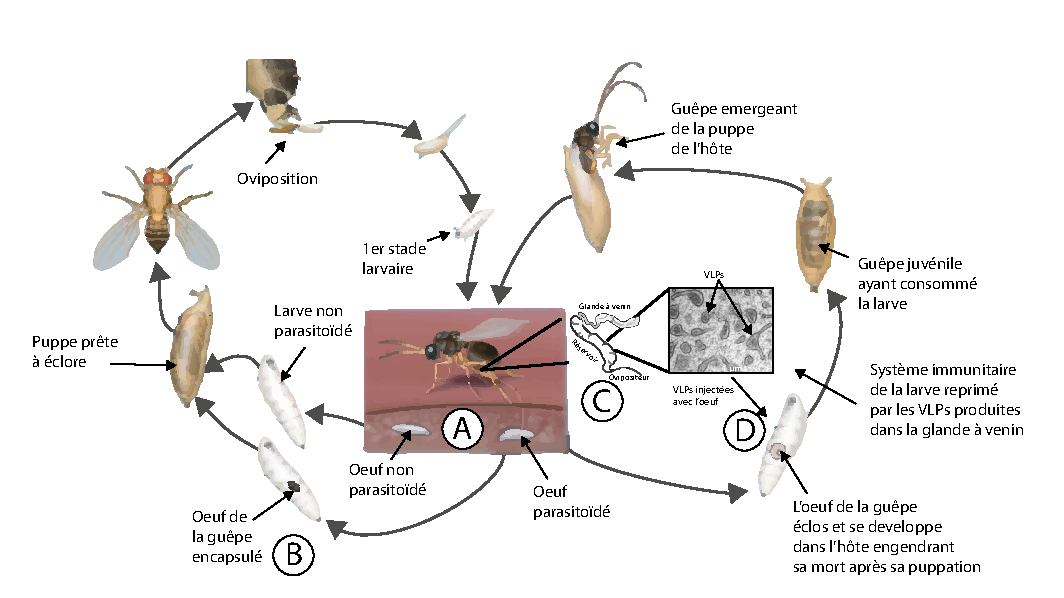
\includegraphics[width=\linewidth,height=\textheight,keepaspectratio]{PhD-master/figures/Leptopilina_lifecycle.pdf}
\caption[Intro:Récapitulatif du cycle de vie d'une espèce de \textit{Leptopilina}]{\textbf{Récapitulatif du cycle de vie d'une espèce de \textit{Leptopilina} modifié à partir du poster d'Amy C. Driskell et al.}}
\label{figure:Leptopilina_lifecycle}
\end{figure}


Aussi, face à cette réponse de l'hôte, les \textit{Leptopilina} ont également trouvé des stratégies pour empêcher l'élimination de leurs œufs. L'une de ces stratégies implique en effet la domestication de gènes viraux qui permettent de produire des VLPs (Virus-like particules) \citep{rizki_parasitoid_1990}. Ces VLPs sont produites dans la glande à venin de la guêpe et sont dépourvues d'ADN, mais contiennent plutôt des protéines de virulence (\figurename{\ref{figure:Leptopilina_lifecycle}}-C). Ces VLPs sont injectées au côté de l'œuf dans la larve de drosophile \citep{colinet_convergent_2007} (\figurename{\ref{figure:Leptopilina_lifecycle}}-D). Une fois injectées dans l'hôte de la guêpe, les VLPs délivrent leur contenu dans les lamellocytes (cellules impliquées dans l'encapsulation) de l'hôte, ce qui modifie principalement leur forme en affectant le cytosquelette, rendant incapable la cellule d'adhérer à l'œuf de parasitoïde \citep{rizki_parasitoid_1990, colinet_convergent_2007} (\figurename{\ref{figure:Leptopilina_VLPs}} - figure en bas à droite). De plus, il a été montré que l'infestation par \textit{L. heterotoma}/ \textit{L. victoriae} provoque également l'apoptose des hémocytes \citep{chiu_natural_2002}.

%\begin{figure}[!htpbt]
%\captionsetup{font=footnotesize}
% \centering
%  \includegraphics[width=\linewidth,height=\textheight,keepaspectratio]{PhD-master/figures/Naldaviricetes_phylogeny.pdf}
%\caption[Intro:Phylogénie des \textit{Naldaviricetes}]{\textbf{Phylogénie des \textit{Naldaviricetes}}}
%\label{figure:Naldaviricetes_phylogeny}
%\end{figure}


L'ancêtre viral responsable de la production de VLPs chez les espèces du genre \textit{Leptopilina} a été récemment identifié comme un proche parent d'un virus filamenteux observé chez \textit{L. boulardi} (LbFV) (Di Giovanni et al., 2020). Parmi les milliers de gènes présents dans le génome de trois espèces (\textit{L.boulardi}, \textit{L.heterotoma} et \textit{L.clavipes}), 13 présentaient des homologies de séquences convaincantes avec 13 ORFs du génome de LbFV. Ces 13 éléments viraux endogènes (EVEs) proviennent très probablement du même événement d'endogénisation ancestral, car leur distribution le long des génomes de trois espèces de \textit{Leptopilina} comprend quelques blocs synténiques et la phylogénie des gènes est parfaitement congruente avec celles des espèces (Di Giovanni et al., 2020) (\figurename{\ref{figure:Leptopilina_VLPs}}). Ces EVEs sont spécifiquement exprimés dans la glande à venin au début du stade nymphal, lorsque les VLPs sont synthétisées. Chose surprenante par rapport aux cas déjà connus chez les polydnavirus  d'Ichneumonoidea, l'amplification génomique d'une partie des EVEs  (10/13) est vraisemblablement régie par une ADN polymérase virale (LbFV\_ORF58) ce qui  entraîne une modulation de leur profil d'expression (\figurename{\ref{figure:Leptopilina_VLPs}}) (Di Giovanni et al., 2020). Plusieurs de ces gènes codent des protéines ayant des fonctions connues chez les virus, dans la transcription (\textit{lef-4}, \textit{lef-8}, et \textit{lef-9}), la réplication de l'ADN (\textit{DNApol}, \textit{helicase}), l'enveloppement des protéines de virulence (\textit{ac81}), et la formation de membranes lipidiques (\textit{lcat}). De plus, l'absence des gènes nécessaires à la production de la capside est cohérente avec l'absence de capside chez les VLPs. Comme on pourrait s'y attendre, les 13 EVEs sont tous soumis à une forte pression de sélection purificatrice (\textit{dN/dS} << 1). De plus, l'un de ces EVEs (LbFV\_ORF85) a été retrouvé par des approches de protéomiques dans les VLPs purifiés, ce qui corrobore leur implication dans leur production (Di Giovanni et al., 2020). Ces VLPs, chez \textit{L.boulardi} ont un rôle essentiel dans le succès reproducteur des guêpes puisqu'ils désactivent les lamellocytes de l'hôte en modifiant leur morphologie  \citep{rizki_parasitoid_1990, colinet_convergent_2007} (\figurename{\ref{figure:Leptopilina_VLPs}}).

\begin{figure}[!htpbt]
\captionsetup{font=footnotesize}
 \centering
  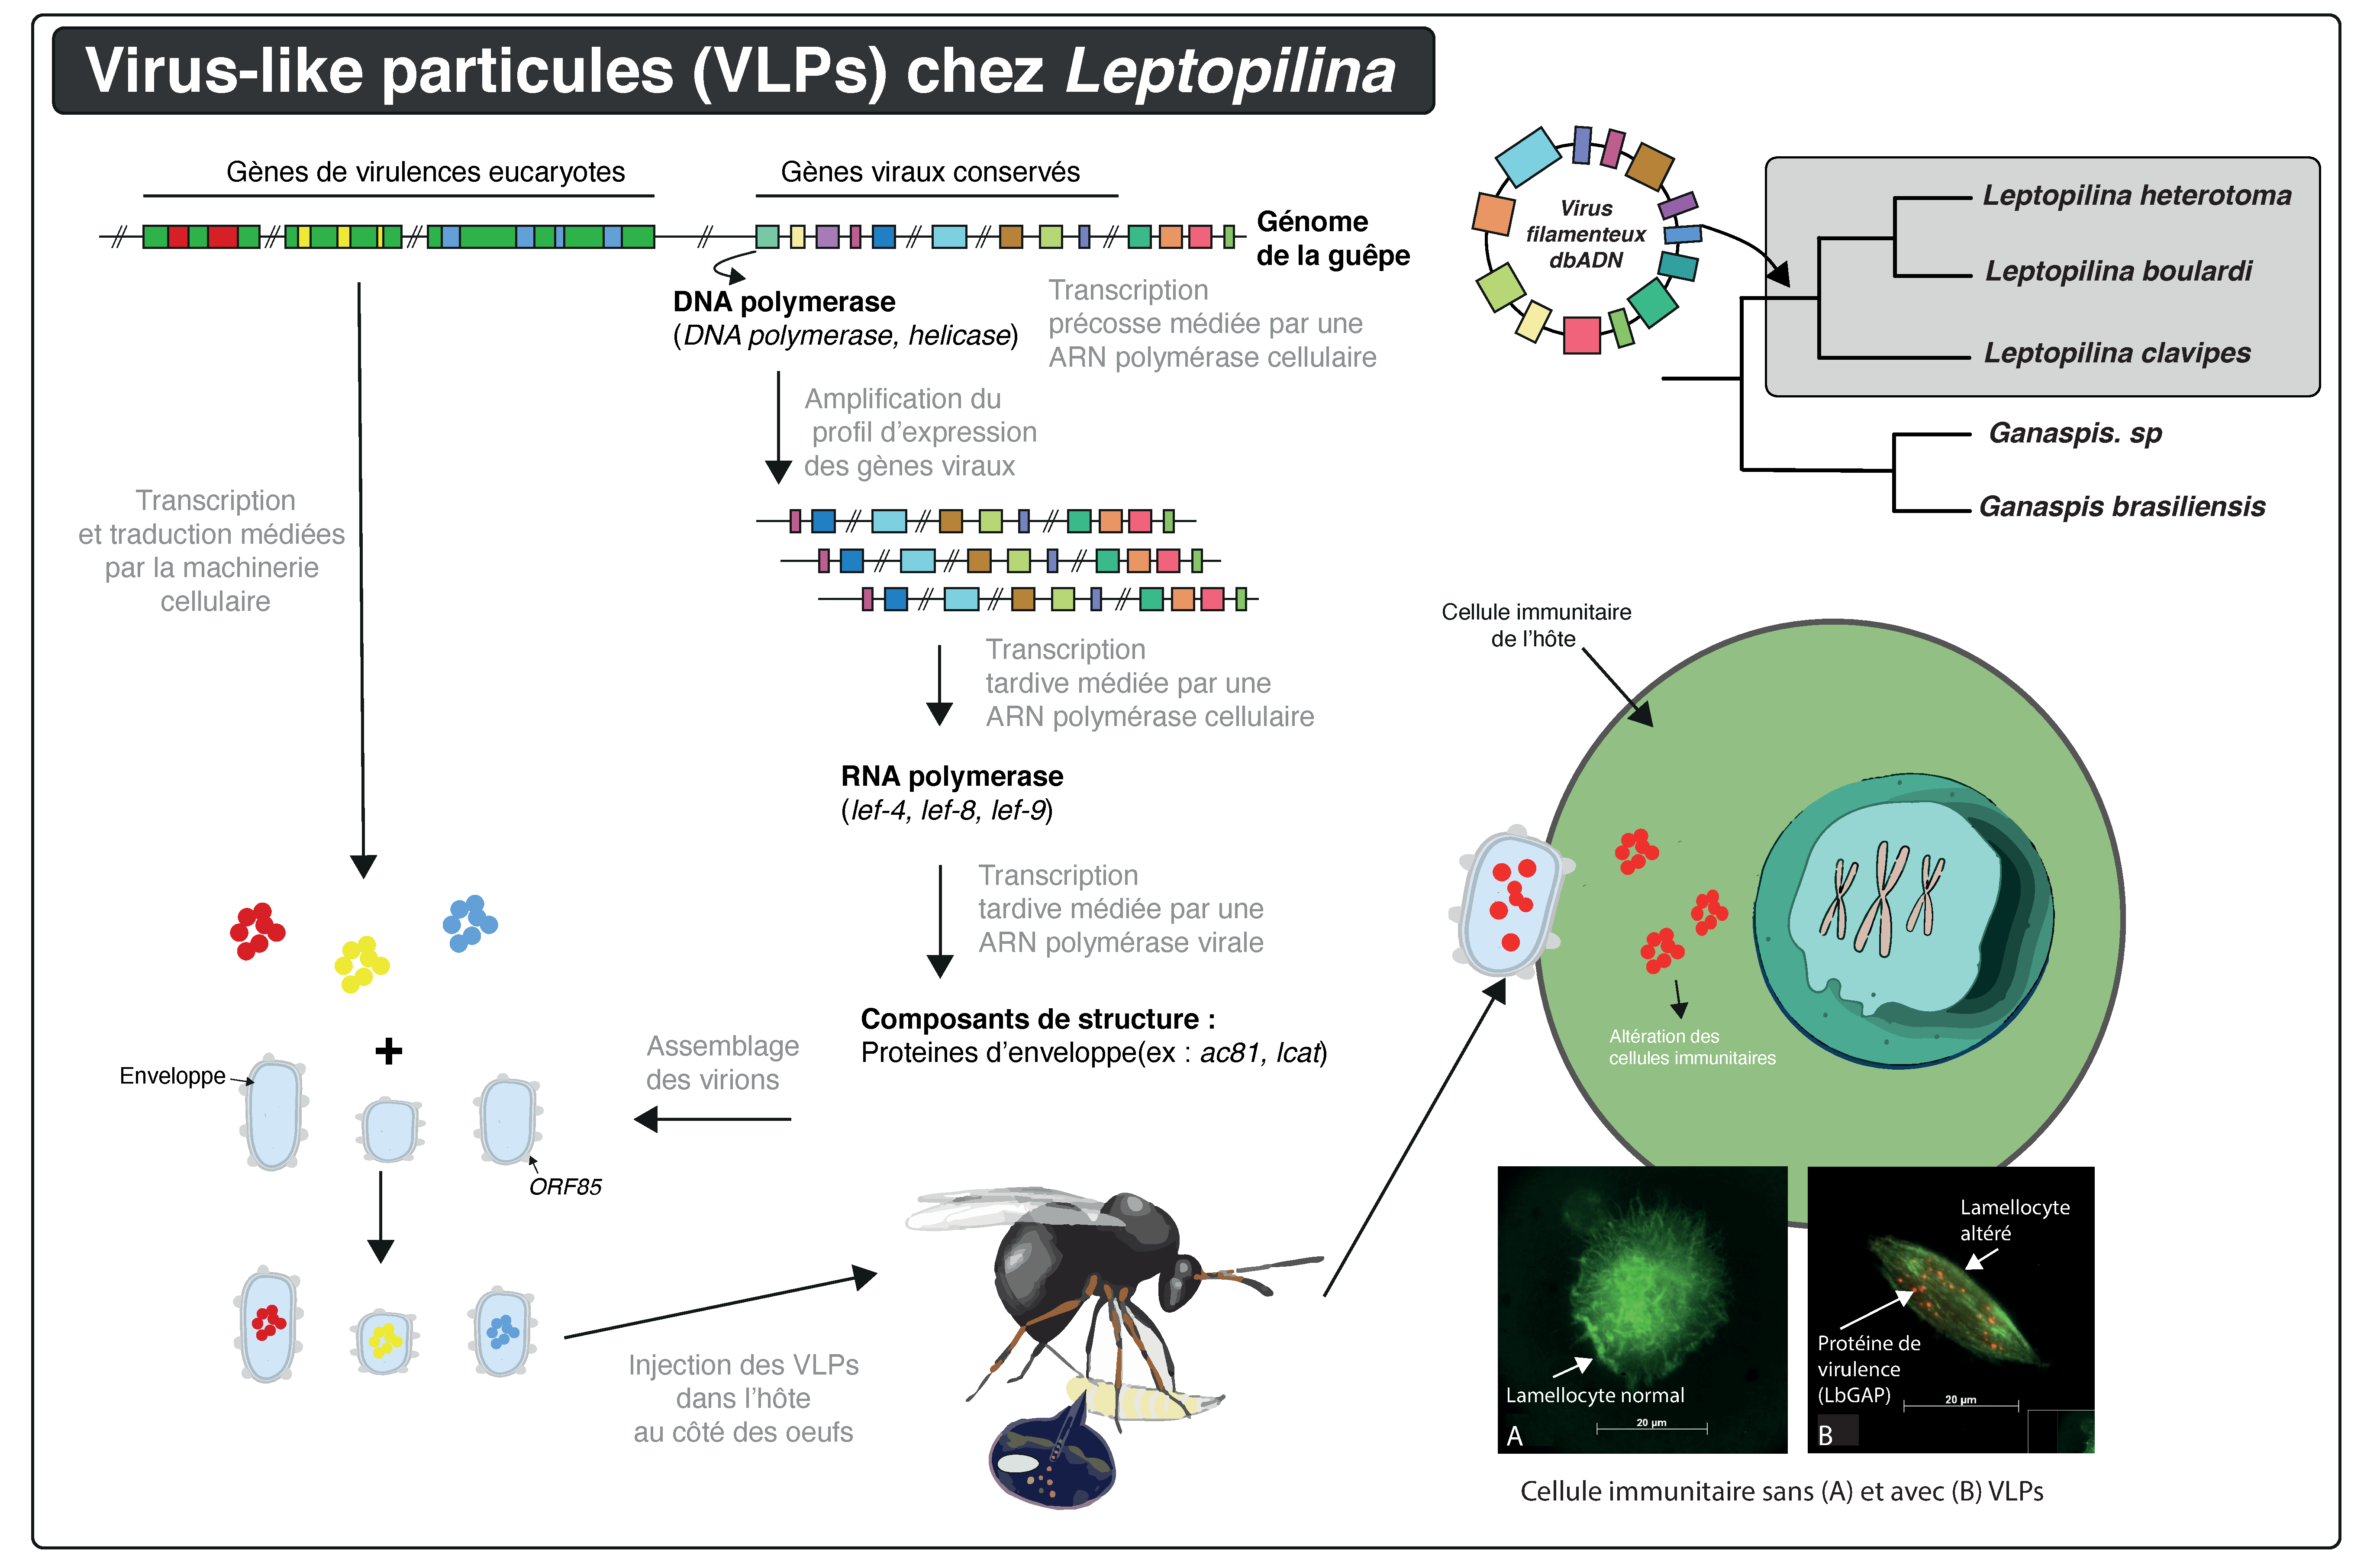
\includegraphics[width=\linewidth,height=\textheight,keepaspectratio]{PhD-master/figures/Leptopilina_VLPS.pdf}
\caption[Intro:Récapitulation du fonctionnement putatif des VLPs chez les espèces de \textit{Leptopilina}]{\textbf{Récapitulation du fonctionnement putatif des VLPs chez les espèces de \textit{Leptopilina}} (photo de \cite{colinet_convergent_2007})}
\label{figure:Leptopilina_VLPs}
\end{figure}

Jusqu'à présent, tous les membres du genre \textit{Leptopilina} (6 examinés) se sont révélés positifs pour la présence d'EVEs homologues à des ORFs de LbFV et produisent toutes des VLPs pour protéger leurs descendants (Di Giovanni et al., 2020). D'autres espèces éloignées des \textit{Leptopilina} mais de la même sous-famille (Eucoilinea) du genre \textit{Ganaspis} (Di Giovanni et al., 2020) n'ont quant à elles présentées aucune homologie avec des ORFs de LbFV et aucun VLPs n'ont été décrits (\figurename{\ref{figure:Figitidae_diversity_intro}}).

\begin{figure}[H]
\captionsetup{font=footnotesize}
 \centering
  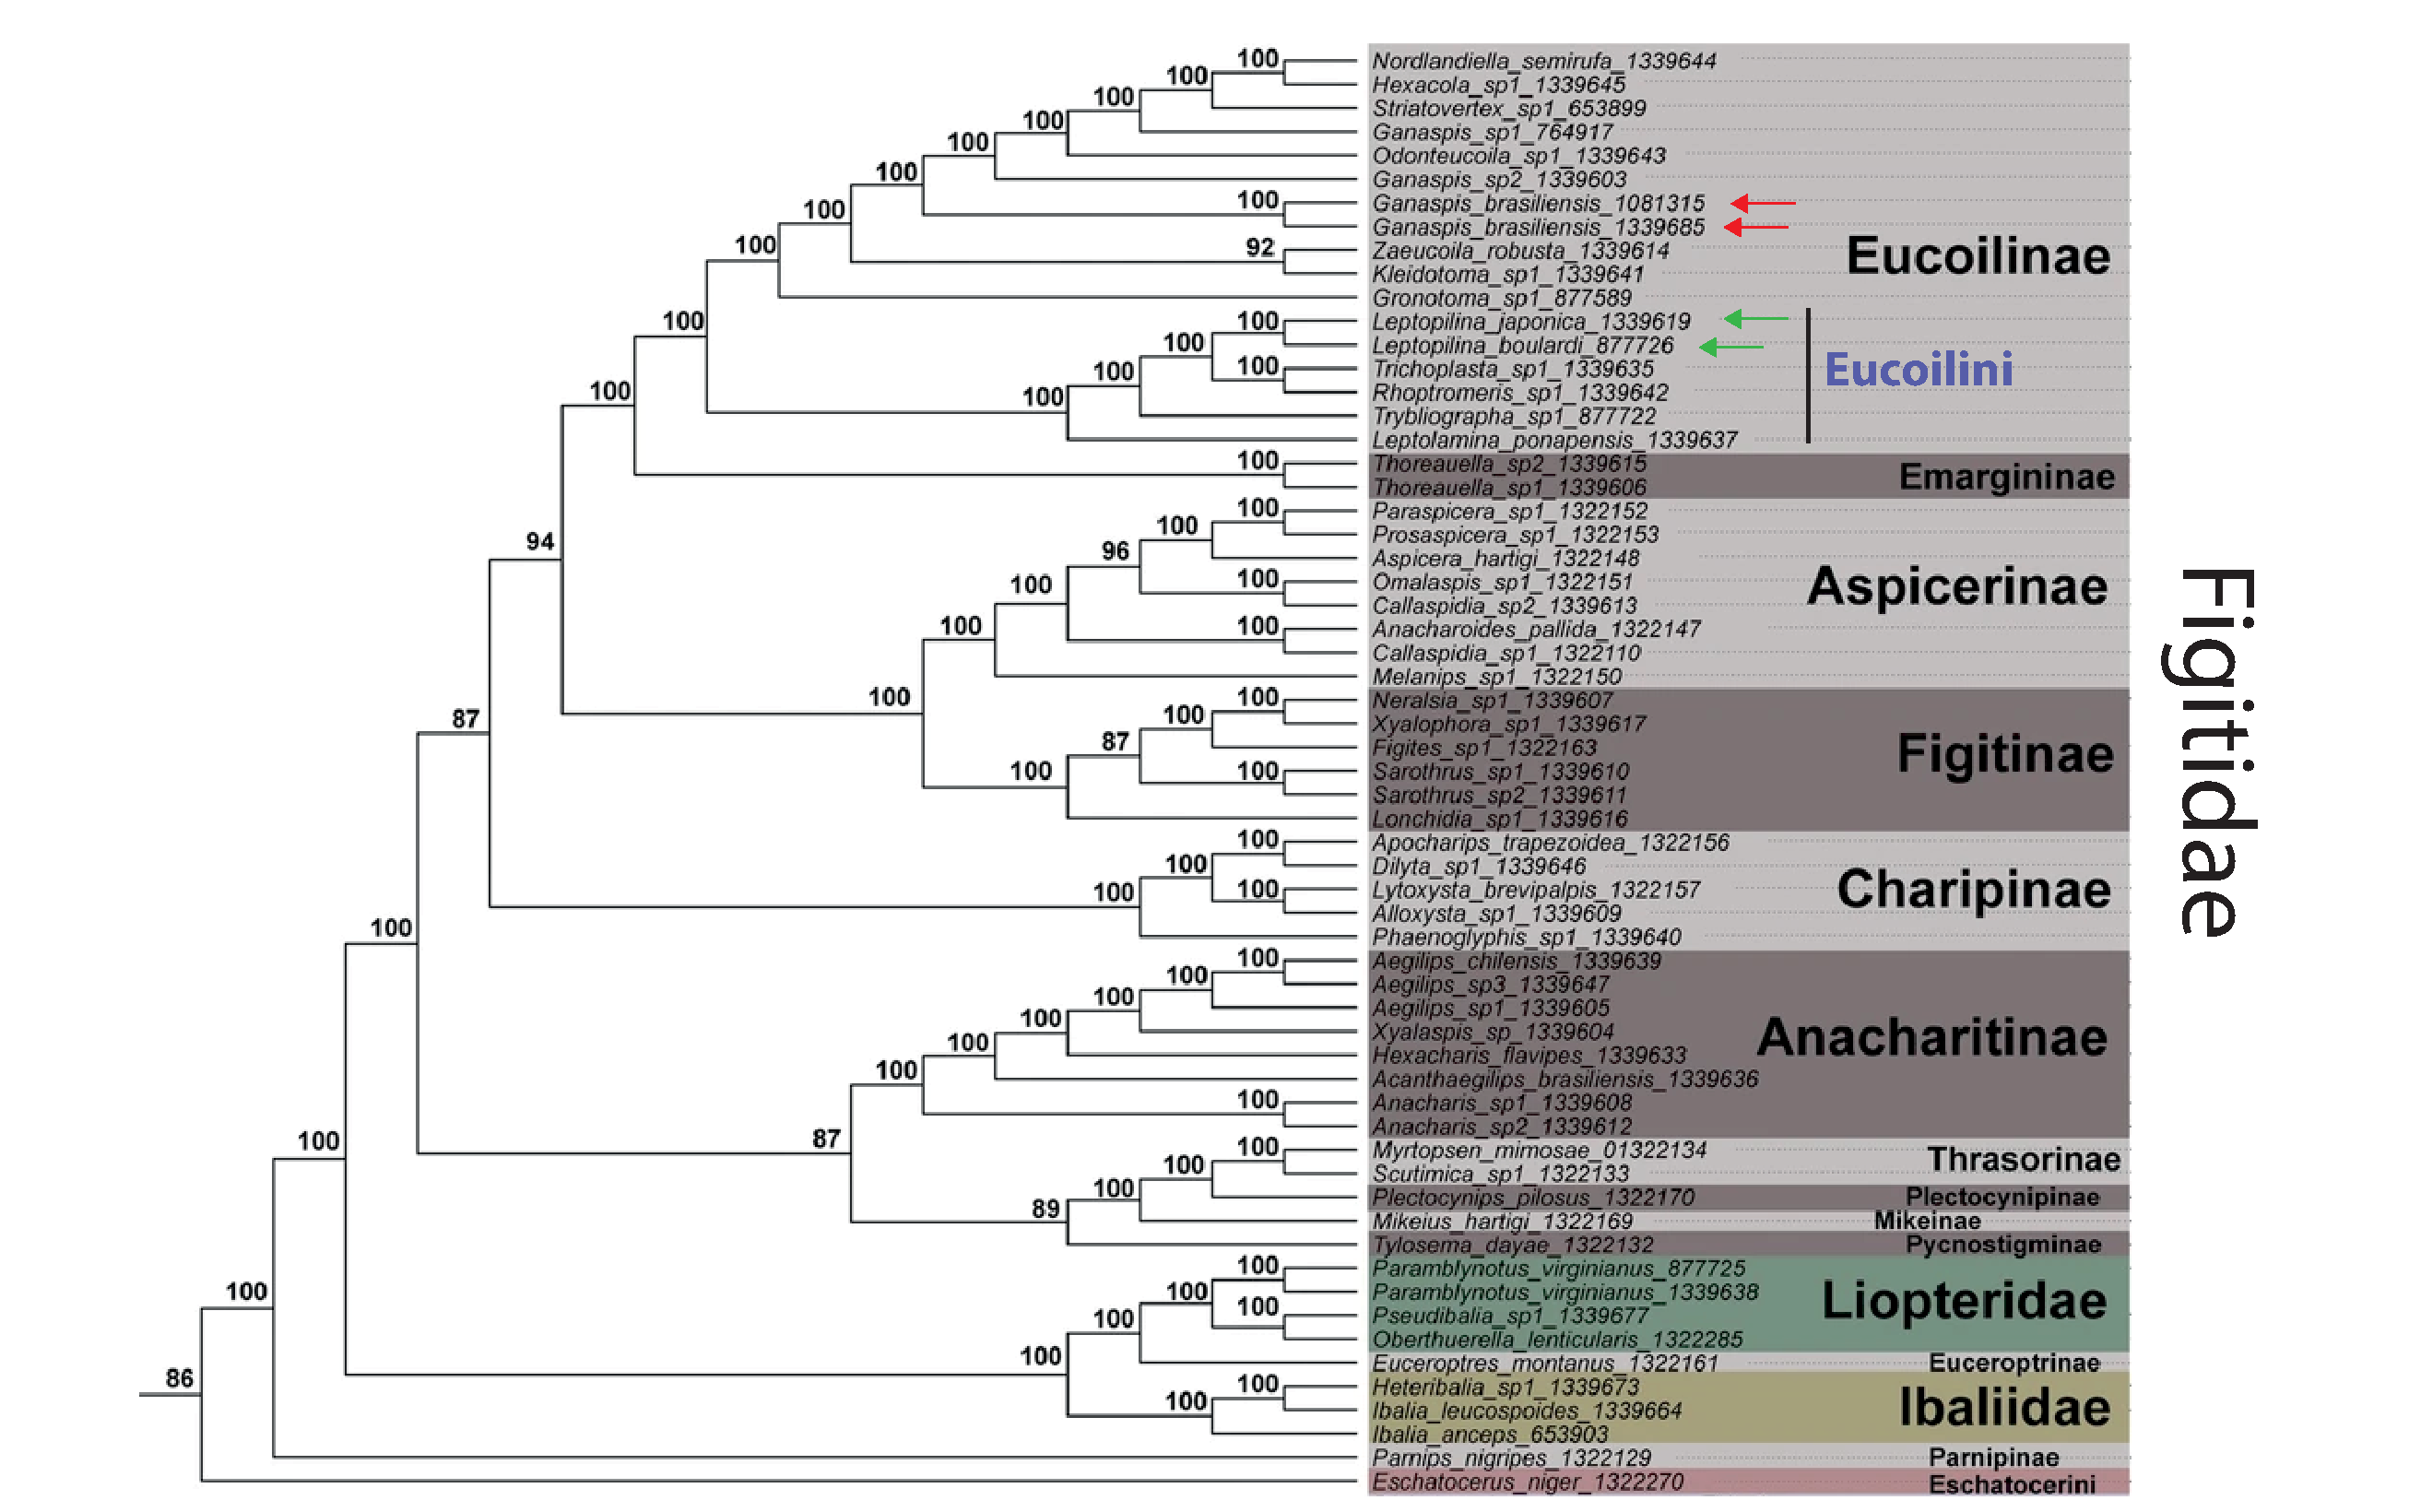
\includegraphics[width=\linewidth,height=\textheight,keepaspectratio]{PhD-master/figures/Figitidae_diversity_intro.pdf}
\caption[Intro:Arbre phylogénétique de la diversité des espèces de la famille des Figitidae]{\textbf{Arbre phylogénétique de la diversité des espèces de la famille des Figitidae}. Les flèches vertes correspondent à la présence d'EVEs homologues à LbFV tandis que les flèches rouges correspondent à l'absence d'homologie (source de \cite{blaimer_comprehensive_2020})}
\label{figure:Figitidae_diversity_intro}
\end{figure}

D'autres EVEs putatifs liés au LbFV ont été trouvés chez d'autres espèces endoparasitoïdes, comme chez \textit{Dolichomitus sp} (Ichneumonidae) \citep{burke_presence_2021} et \textit{Cotesia vestalis} \citep{burke_presence_2021} (\figurename{\ref{figure:Virus_arthropods_phylogeny}}-B), mais ces espèces sont trop éloignées des espèces de \textit{Leptopilina} pour faire partie du même événement d'endogénisation, de plus leur caractère intégré n'est pas réellement clair, surtout concernant \textit{Dolichomitus sp} dans lequel une forme intégrée et libre seraient présentes dans les données \citep{burke_endogenization_2020}. Cela signifie donc que l'événement d'endogénisation s'est produit après la divergence de l'ancêtre commun des espèces \textit{Ganaspis} et \textit{Leptopilina}, il y a environ 91 millions d'années \citep{blaimer_comprehensive_2020} et avant la divergence des espèces \textit{Leptopilina}, il y a environ 41,7 millions d'années \citep{blaimer_comprehensive_2020}. 

Au final, nous manquons de détails sur la gamme d'espèces concernées par cet événement, ainsi que sur l'histoire évolutive de ces virus et leur rôle putatif dans l'évolution de des Figitidae.